\documentclass[12pt,a4paper,fancyhdr,openany,oneside]{ctexbook}
\usepackage[colorlinks=true]{hyperref}
\usepackage{listings}
\usepackage{graphicx}
\usepackage{tikz}
\usepackage{flowchart}
\usepackage{float}
\usepackage{amsmath}
\usetikzlibrary{shapes,arrows}
\usetikzlibrary{shapes.geometric, arrows}
\lstset{
    basicstyle          =   \sffamily,          % 基本代码风格
    keywordstyle        =   \bfseries,          % 关键字风格
    commentstyle        =   \rmfamily\itshape,  % 注释的风格,斜体
    stringstyle         =   \ttfamily,  % 字符串风格
    flexiblecolumns,                % 别问为什么,加上这个
    % numbers             =   left,   % 行号的位置在左边
    showspaces          =   false,  % 是否显示空格,显示了有点乱,所以不现实了
    numberstyle         =   \zihao{-5}\ttfamily,    % 行号的样式,小五号,tt等宽字体
    showstringspaces    =   false,
    captionpos          =   t,      % 这段代码的名字所呈现的位置,t指的是top上面
    frame               =   lrtb,   % 显示边框
}

\lstdefinestyle{Python}{
    language        =   Python, % 语言选Python
    basicstyle      =   \zihao{-5}\ttfamily,
    numberstyle     =   \zihao{-5}\ttfamily,
    keywordstyle    =   \color{blue},
    keywordstyle    =   [2] \color{teal},
    stringstyle     =   \color{magenta},
    commentstyle    =   \color{red}\ttfamily,
    breaklines      =   true,   % 自动换行,建议不要写太长的行
    columns         =   fixed,  % 如果不加这一句,字间距就不固定,很丑,必须加
    basewidth       =   0.5em,
}

\begin{document}
%定义流程图的具体形状
\tikzstyle{startstop} = [rectangle,rounded corners, minimum width=3cm,minimum height=1cm,text centered, draw=black,fill=red!30]
\tikzstyle{io} = [trapezium, trapezium left angle = 70,trapezium right angle=110,minimum width=3cm,minimum height=1cm,text centered,draw=black,fill=blue!30]
\tikzstyle{process} = [rectangle,minimum width=3cm,minimum height=1cm,text centered,text width =3cm,draw=black,fill=orange!30]
\tikzstyle{decision} = [diamond,minimum width=3cm,minimum height=1cm,text centered,draw=black,fill=green!30]
\tikzstyle{arrow} = [thick,->,>=stealth]


\tableofcontents


\chapter{绪论}
\section{选题背景及意义}
\section{当前领域的研究现状}
\section{论文主要工作和内容}

\chapter{关键技术介绍与分析}
\section{本章概要}
\section{Django开发框架概述}
\section{Neo4J图数据库概述}
\section{跨模态视频检索技术概述}
\section{语音识别技术概述}
\section{知识图谱技术概述}
\section{本章小结}



\chapter{跨膜态搜索系统需求分析}
\section{本章概要}
\section{系统可行性分析}
对软件系统的可行性分析是软件开发流程中不可或缺的一部分。可行性分析主要对即将进行开发的软件项目
在技术、经济和社会因素方面进行可行性的评估,目的是为了合理的制定目标和论证选定设计方案的理由。\cite{软件项目中的可行性分析方法研究}
本文主要从技术、经济、社会和操作四个角度对本系统进行了研究与分析,分析结果显示本系统的方案可行且具备一定的经济效益和社会效益。


\subsection{技术可行性}
基于知识图谱的文本-视频跨膜态搜索系统主要应用场景在Web端。得益于近年来互联网技术的发展,各种Web技术蓬勃发展、体系日渐完善,
本文服务端采用Python语言,使用Django框架编写服务端功能。使用JavaScript语言和Vue前端框架来完成UI的功能实现。
由于Python语言开发的机器学习相关算法的生态比较成熟,所以本文语言识别和知识图谱相关的算法实现也采用Python。而且这些算法
在学术界都有丰富可靠的理论研究。尤其有如TensorFlow、Pytorch等框架的出现给机器学习算法的实现降低了门槛,并有活跃的社区可供开发人员参考和学习,
为项目的敏捷开发和快速迭代起到了关键作用。综上所述本文所设计的系统在技术上可行。

\subsection{经济可行性}
经济可行性分析是指一个新的软件开发项目在经济角度评估是否可行,它主要是投入产出比(ROI)的分析。本文系统采用的技术均是开源的框架技术及开源
数据库,所以主要是人力和时间成本,对于提供视频内容业务的互联网企业来说,其成本在可控范围内。而且本文的系统弥补了目前市场视频跨膜态搜索的一个缺口,
因此在经济上是有巨大盈利的期望的。所以本文所设计的系统在经济上可行。

\subsection{社会可行性}
社会环境的可行性包括了两种因素:市场与政策。\cite{软件项目中的可行性分析方法研究}

其中市场又可以分为未成熟的市场、成熟的市场和将要消亡的市场,
政策主要涉及到法律和知识产权。

环境分析就是明确系统的目的和限制条件:使用单位的状况、经营方针和组织机构、使用单位
的计算机利用情况:相关的硬件、软件及其它接口部分;用户的
操作环境及操作要求;习惯、法律、制度上对软件的制约;开发能
具备的基数条件和设备条件。



\section{系统总体业务分析}

\section{系统功能性需求分析}
\subsection{系统角色模块分析}
\subsection{视频上传模块需求分析}
\subsection{视频语音识别模块需求分析}
\subsection{知识图谱构建模块需求分析}
\subsection{视频搜索模块需求分析}


\section{系统非功能性需求分析}
\paragraph{系统的安全性}asdf
\paragraph{系统的可维护性}asdf
\paragraph{系统的易用性}asdf
\paragraph{系统的可扩展}asdf
\section{本章小结}
% 
\chapter{文本-视频跨膜态搜索系统的设计}
\section{本章概要}
\section{系统技术架构设计}
\section{系统功能模块设计}
\subsection{系统角色模块设计}
\subsection{视频上传模块设计}
\subsection{视频语音识别模块设计}
\subsection{知识图谱构建模块设计}
\subsection{视频搜索模块设计}
\section{数据库设计}
\section{本章概要}







% 
\chapter{文本-视频跨膜态搜索系统的设计}
\section{本章概要}
\section{语音转文字算法的设计}
\subsection{问题描述}
问题描述,问题描述,问题描述,问题描述,问题描述。
\subsection{算法设计与实现}
\subsubsection{算法总体流程} 
本算法对音频文件先进行特征提取得到语谱图,之后直接将语谱图输入声学模型将声音转录为中文拼音,
最后通过统计语言模型,将拼音序列转换为中文文本,流程图如\ref{flowchart}所示。
\begin{figure}[htbp]
    \centering
        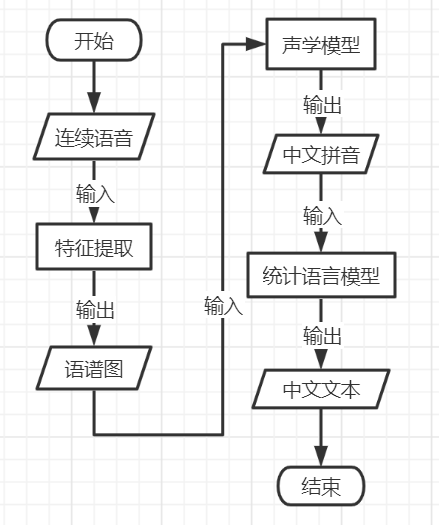
\includegraphics[width=0.4\textwidth]{resource/img/flowchart.png}
        \caption{算法流程}
        \label{flowchart}
\end{figure}

语谱图(spectrogram)也称语音频谱图。一般是通过处理接收的时域信号得到频谱图,
因此只要有足够时间长度的时域信号就可。语谱图的特点是观察语音不同频段的信号强度,可以看出随时间的变化情况。
本文就是通过将语谱图作为特征输入,利用CNN进行图像处理进行训练。

声学模型结构上,用深度学习的方法并借鉴了图像识别中效果最好的网络配置VGG,这种网络模型有着很强的表达能力,
可以看到非常长的历史和未来信息,相比RNN在鲁棒性上更出色。
在输出端,本文将声学模型结合定义好的CTC损失函数来进行训练,以实现整个模型的端到端训练,将声音波形信号直接转录为中文
普通话拼音序列。

直接将一句语音转化成一张图像作为输入,即先对每帧语音进行傅里叶变换,再将时间和频率作为图像的两个维度,然后通过非常多的卷积层和池化(pooling)层的组合,对整句语音进行建模,输出单元直接与最终的识别结果比如音节或者汉字相对应。

它借鉴了图像识别中效果最好的网络配置,每个卷积层使用3x3的小卷积核,并在多个卷积层之后再加上池化层,这样大大增强了CNN的表达能力,与此同时,通过累积非常多的这种卷积池化层对,DFCNN可以看到非常长的历史和未来信息,有这两点就保证了DFCNN可以出色的表达语音的长时相关性,相比RNN网络结构在鲁棒性上反而更加出色。最后,从输出端来看,DFCNN还可以和近期很热的序列短时分类(CTC)方案完美结合以实现整个模型的端到端训练,且其包含的池化层等特殊结构可以使得以上端到端训练变得更加稳定。
CTC(Connectionist Temporal Classification)//TODO


本文的语言模型上采用统计语言模型,通过最大熵隐含马尔可夫模型,将拼音序列转换为中文文本。


\paragraph{1.特征提取} 将普通的wav语音信号通过分帧、加窗、快速傅立叶变换(FFT)操作转换为神经网络需要的二维频谱图像信号。

https://blog.ailemon.net/2021/03/08/speech-acoustic-feature-extraction-the-principle-and-implement-of-the-spectrogram-algorithm-for-asrt/
本次算法设计在声学特征的提取上,不是直接采用MFCC算法而是根据传统MFCC算法修改的,提取语谱图。
不过这种语谱图特征也是从MFCC算法修改而来的,目的是保留更多的原始信息以供神经网络计算,
避免经过人工特征设计的滤波器产生大量的信息损失。保留更多的原始信息以供神经网络计算,避免经过人工特征设计的滤波器
产生大量的信息损失。语谱图特征是有别于mfcc和logfBank特征的另一种声学特征,与其说是提取特征,不如说是仅仅对声音信号进行预处理。
传统的MFCC特征、fBank和logfBank等特征在傅里叶变换后,都存在各种类型人工设计的滤波器,如Mel滤波器。
这些基于人工特征算法的语音特征提取,会造成频域中的语音信号,尤其是高频区域的信号,其声音信息的损失会比较大。
而那些传统语音特征提取算法,在时域上还存在着非常大的时间窗偏移,其目的是用来降低运算量,所以也会导致声音信息的损失
问题,尤其是说话人语速较快时[1]。
以下是传统的MFCC特征提取算法的流程,如图\ref{mfcc.png}所示。
\begin{figure}[htbp]
\centering
    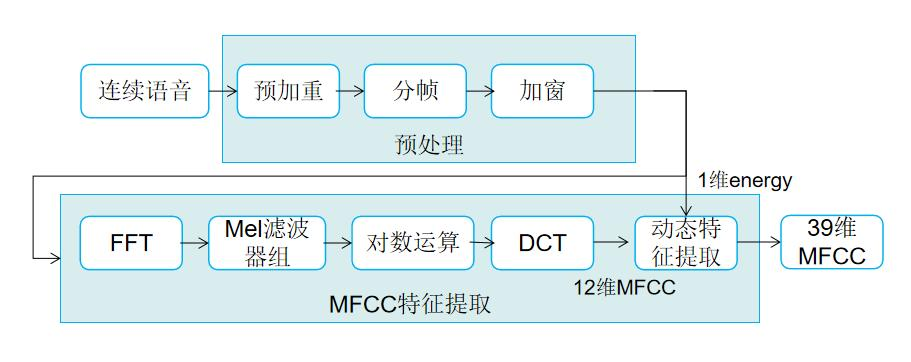
\includegraphics[width=0.8\textwidth]{resource/img/mfcc.png}
    \caption{MFCC算法}
    \label{mfcc.png}
\end{figure}

语谱图则在logfBank特征去掉离散余弦变换的基础上,再去掉人工特征滤波器(Mel滤波器),以及第一步预加重的过程,
直接将快速傅里叶变换并取模之后得到的“时-频”幅度谱取对数,得到的结果作为语音特征的表示。如图\ref{spectrogram.png}。
\begin{figure}[htbp]
    \centering
        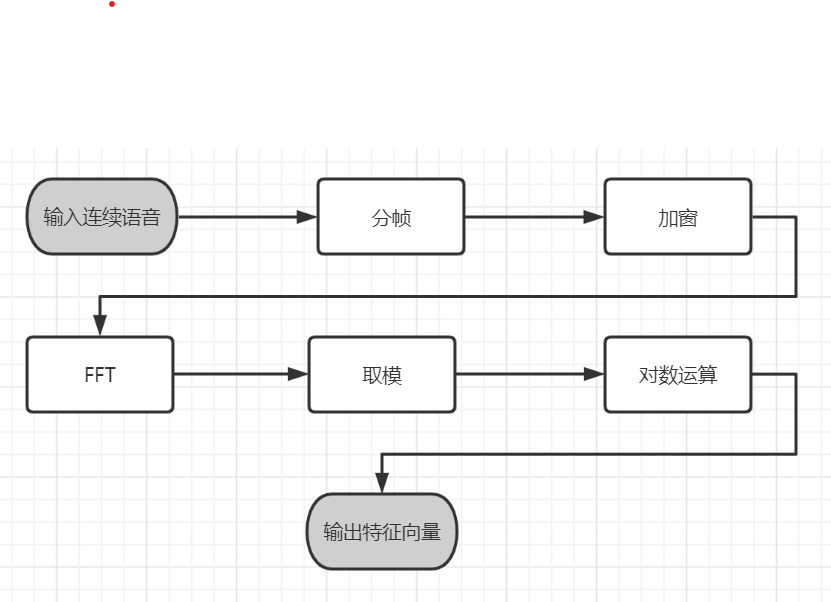
\includegraphics[width=0.8\textwidth]{resource/img/spectrogram.png}
        \caption{语谱图提取}
        \label{spectrogram.png}
\end{figure}

这种不直接经过人工设计的滤波器进行特征提取,得到“时域-频域”的对数幅度谱,就是我们这里所说的语谱图。
这种特征的好处是将进一步的特征提取交给后续的神经网络模型来实现,神经网络可以在训练的过程中,自动学习到类似Mel滤波器
的提取特征,由于包含了更多传统算法丢掉的信息,所以本算法在此系统的实际应用中,效果优于传统特征提取算法。


\subparagraph{1.1 读取音频} 第一步,我们需要找到利用scipy模块将音频转化为有用的信息, fs 为采样频率,
wavsignal为语音数据。我们的数据集的fs均为16khz,代码如下\ref{importWavFile.py}。
\begin{lstlisting}[style=Python,
    caption={importWavFile.py},
    label={importWavFile.py}]
    import scipy.io.wavfile as wav
    filepath = 'test.wav'
    fs, wavsignal = wav.read(filepath)
\end{lstlisting}


\subparagraph{1.2 分帧、加窗} 
语音信号在宏观上是不平稳的,在微观上是平稳的,具有短时平稳性(10—30ms内可以认为语音信号近似不变为一个音素的发音,
一般情况下取 25ms 。为了处理语音信号,我们要对语音信号进行加窗,也就是一次仅处理窗中的数据。
因为实际的语音信号是很长的,我们不能也不必对非常长的数据进行一次性处理。明智的解决办法就是每次取一段数据,
进行分析,然后再取下一段数据,再进行分析。我们的加窗操作指的就是汉明窗操作,
原理就是把一帧内的数据乘以一个函数$ W\left ( n \right ) $,并得到新的一帧数据。
怎么仅取一段数据呢?因为之后我们会对汉明窗中的数据进行快速傅立叶变换(FFT),它假设一个窗内的信号是代表一个周期的
信号(也就是说窗的左端和右端大致可以连续),而通常一小段音频数据没有明显的周期性,加上汉明窗后,数据就比较接近周期函数了。
由于加上汉明窗,只有中间的数据体现出来了,两边的数据信息丢失了,所以等会移窗的时候会有重叠的部分,当窗口取了 25ms 时,
步长可以取 10ms (其中 a 的值一般取0.46)。公式为:\ref{hanmming}

\begin{displaymath}
        W\left ( n,a \right ) = \left ( 1-a \right )-a*cos\left [ \frac{2n}{N-1} \right ], 0\leq n\leq N-1 
\end{displaymath}
\begin{equation}
    \label{hanmming}
        S' \left ( n \right ) = S\left ( n \right )*W\left ( n \right )
\end{equation}
代码实现如\ref{framing.py}所示
\begin{lstlisting}[style=Python, caption={framing.py}, label={framing.py}]
    import numpy as np
    x=np.linspace(0, 400 - 1, 400, dtype = np.int64)#返回区间内的均匀数字
    w = 0.54 - 0.46 * np.cos(2 * np.pi * (x) / (400 - 1))
    time_window = 25
    window_length = fs // 1000 * time_window

    # 分帧
    p_begin = 0
    p_end = p_begin + window_length
    frame = wavsignal[p_begin:p_end]
    plt.figure(figsize=(15, 5))
    ax4 = plt.subplot(121)
    ax4.set_title('the original picture of one frame')
    ax4.plot(frame)

    # 加窗
    frame = frame * w
    ax5 = plt.subplot(122)
    ax5.set_title('after hanmming')
    ax5.plot(frame)
    plt.show() # 分帧、加窗的输出
\end{lstlisting}
图片为效果为\ref{framing.png}
\begin{figure}[htbp]
    \centering
        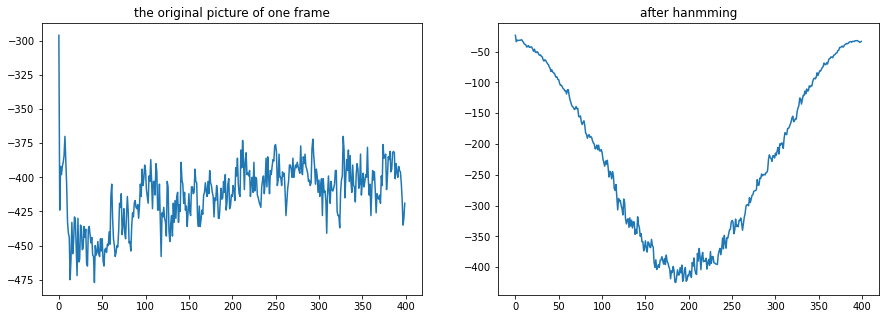
\includegraphics[width=0.8\textwidth]{resource/img/framing.png}
        \caption{分帧、加窗的输出}
        \label{framing.png}
\end{figure}


\subparagraph{1.3 快速傅立叶变换 (FFT)}
语音信号在时域上比较难看出其特性,所以通常转换为频域上的能量分布,所以我们对每帧经过窗函数处理的信号做快速傅立叶变换将时域图转换成各帧的频谱,
然后我们可以对每个窗口的频谱叠加得到语谱图。代码为:\ref{fft.py}
\begin{lstlisting}[style=Python, caption={fft.py}, label={fft.py}]
    from scipy.fftpack import fft
    # 进行快速傅里叶变换
    frame_fft = np.abs(fft(frame))[:200]
    plt.plot(frame_fft)
    plt.show()
    # 取对数,求db
    frame_log = np.log(frame_fft)
    plt.plot(frame_log)
    plt.show() #快速傅立叶变换的输出
\end{lstlisting}
图片为效果为
\begin{figure}[htbp]
    \centering
        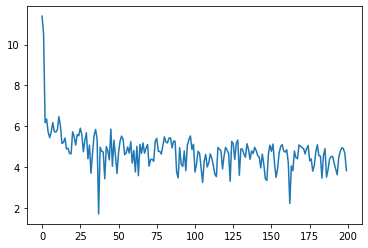
\includegraphics[width=0.8\textwidth]{resource/img/fft.png}
        \caption{快速傅立叶变换的输出}
        \label{fft.png}
\end{figure}





\paragraph{2.声学模型}
基于Keras和TensorFlow框架,使用这种参考了VGG的深层的卷积神经网络作为网络模型并训练。
\paragraph{3.CTC解码}https://yudonglee.me/ctc-explained/
在语音识别系统的声学模型的输出中,往往包含了大量连续重复的符号,因此,我们需要将连续相同的符合合并为同一个符号,
然后再去除静音分隔标记符,得到最终实际的语音拼音符号序列。\cite{hannun2017sequence}

谈及语音识别,如果这里有一个剪辑音频的数据集和对应的转录,而我们不知道怎么把转录中的字符和音频中的音素对齐,
这会大大增加了训练语音识别器的难度。如果不对数据进行调整处理,那就意味着不能用一些简单方法进行训练。对此,
我们可以选择的第一个方法是制定一项规则,如“一个字符对应十个音素输入”,但人们的语速千差万别,这种做法很容易出现纰漏。
为了保证模型的可靠性,第二种方法,即手动对齐每个字符在音频中的位置,训练的模型性能效果更佳,因为我们能
知道每个输入时间步长的真实信息。但它的缺点也很明显——即便是大小合适的数据集,这样的做法依然非常耗时。
事实上,制定规则准确率不佳、手动调试用时过长不仅仅出现在语音识别领域,其它工作,如手写识别、在视频中添加动作标记,
同样会面对这些问题。这种场景下,正是 CTC 用武之地。 CTC 是一种让网络自动学会对齐的好方法,十分适合语音识别和书写识别。
为了描述地更形象一些,我们可以把输入序列(音频)映射为$X=[x_1,x_2,…,x_T]$,其相应的输出序列(转录)即为$Y=[y_1,y_2,…,y_U]$。
这之后,将字符与音素对齐的操作就相当于在$X$和$Y$之间建立一个准确的映射,详细内容可见CTC经典文章https://distill.pub/2017/ctc/。

对比传统的分类方法,时序分类有如下难点:

$X$和$Y$的长度都是变化的;
$X$和$Y$的长度是不相等的;
对于一个端到端的模型,我们并不希望手动设计$X$和$Y$的之间的对齐。
CTC提供了解决方案,对于一个给定的输入序列$X$,CTC给出所有可能的$Y$的输出分布。
根据这个分布,我们可以输出最可能的结果或者给出某个输出的概率。


Connectionist Temporal Classification(CTC)[1]是Alex Graves等人在ICML 2006上提出的一种端到端的RNN训练方法,
它可以让RNN直接对序列数据进行学习,而无需事先标注好训练数据中输入序列和输入序列的映射关系,使得RNN模型在语音识别等序列学习
任务中取得更好的效果,在语音识别和图像识别等领域CTC算法都有很比较广泛的应用。
总的来说,CTC的核心思路主要分为以下几部分:
\begin{enumerate}
    \item 它扩展了RNN的输出层,在输出序列和最终标签之间增加了多对一的空间映射,并在此基础上定义了CTC Loss函数
    \item 它借鉴了HMM(Hidden Markov Model)的Forward-Backward算法思路,利用动态规划算法有效地计算CTC Loss函数及其导数,从而解决了RNN端到端训练的问题
    \item 最后,结合CTC Decoding算法RNN可以有效地对序列数据进行端到端的预测
\end{enumerate}


对于语音识别,我们有一个声音片段和对应校正后的转写文本数据集。不幸的是,我们不知道如何将文字记录中的字符与音频对齐,这使得训练语音识别器比最开始想的看起来更难。
当然我们可以简单设计一些规则,比如“一个字符对应一段固定时间的音频输入”。但是每个人的说话速度都不一样,这种规则在大多数
情况下会失效。当然我们可以选择将每个字符在音频中的位置手动对其,这在数据集小的情况下是非常管用的,但是对于任何稍大规模的数据集,这种方法
虽然精准但必然非常耗时。许多seq2seq的问题都存在这个难点。不过xxx提出的CTC算法特别适合解决这种问题。
连结时序分类 (CTC) 是一种不知道输入和输出之间的对齐方式。CTC 是一种让网络自动学会对齐的好方法,十分适合语音识别和书写识别。
为了描述地更形象一些,我们可以把输入序列(音频)映射为$X=[x_1,x_2,…,x_T]$,其相应的输出序列(转录)即为$Y=[y_1,y_2,…,y_U]$。这之后,
将字符与音素对齐的操作就相当于在$X$和$Y$之间建立一个准确的映射,




TensorFlow内置了CTC的loss和CTC的beam搜索函数。
损失函数:对于给定的输入,我们希望训练我们的模型以最大化它对齐到正确答案的概率。 为此,我们需要有效地计算条件概率p(Y | X)。 函数p(Y | X)也应该是可微的,所以我们可以使用梯度下降。
损失函数部分代码:\ref{ctcLambda.py}

\begin{lstlisting}[style=Python, caption={ctcLambda.py}, label={ctcLambda.py}]
    from tensorflow.keras import backend as K
    def ctc_lambda(args):
    '''
    y_true:包含真值标签的张量(样本,最大字符串长度)。
    y_pred:包含softmax预测或输出的张量(样本、时间步长、num_类别)。
    input_length:张量(samples,1),包含y_pred中每个批次项目的序列长度。
    label_length:张量(samples,1)包含y_true中每个批次项目的序列长度。
    '''
        labels, y_pred, input_length, label_length = args
        y_pred = y_pred[:, :, :]
        return K.ctc_batch_cost(labels, y_pred, input_length, label_length)
\end{lstlisting}
解码部分代码:\ref{decodeCtc.py}
\begin{lstlisting}[style=Python, caption={decodeCtc.py}, label={decodeCtc.py}]
    #num_result为模型预测结果,num2word 对应拼音列表。
    def decode_ctc(num_result, num2word):
        result = num_result[:, :, :]
        in_len = np.zeros((1), dtype = np.int32)
        in_len[0] = result.shape[1];
        r = K.ctc_decode(result, in_len, greedy = True, beam_width=10, top_paths=1)
        r1 = K.get_value(r[0][0])
        r1 = r1[0]
        text = []
        for i in r1:
            text.append(num2word[i])
        return r1, text
\end{lstlisting}

\paragraph{4.语言模型} 使用统计语言模型,将拼音转换为最终的识别文本并输出。

统计语言模型描述了一串文字序列成为句子的概率。

\subparagraph{4.1 建立模型}
xxx贾里尼克提出了用一个统计模型来判断一个句子是否合乎语法、语义清晰的办法。一个句子是否合理,就看它出现的可能性大小如何。
至于可能性就用概率来衡量。如果$S$是一个有意义的句子,有一连串的词$w_1,w_2,…,w_n$构成(n为句子长度),那么文本$S$成立的可能性,
即概率$P\left ( S \right )$。
我们知道$S=w_1,w_2,…,w_n$, 那么$P\left ( S \right )$就应该是:\ref{ps.eq}
\begin{displaymath}
    P\left ( S \right ) = P\left ( w_1,w_2,…,w_n \right ) 
\end{displaymath}
\begin{equation} \label{ps.eq}
    = P\left ( w_1 \right ) * P\left ( w_2|w_1 \right ) * P\left ( w_3|w_1, w_2\right ) ...
    *P\left ( w_n|w_1, w_2,...,w_{n-1}\right )
\end{equation}
其中$P\left ( w_1 \right )$表示第一个词$w_1$出现的概率,$P\left ( w_2|w_1 \right ) $是在已知第一个词的前提下,第二个词
出现的概率,以此类推,词$w_n$出现的概率取决于它前面的所有词。虽然一个句子的前几个词概率不难计算,但是越往后条件概率$P\left ( w_n|w_1, w_2,...,w_{n-1}\right )$
可能性太多,计算难度太大。但是,这里当前面依赖的词数太多时,模型的产生和正向计算的计算量将非常的大,非常难算,而且计算机的存储空间也有限,每个变量的
可能性都将是一种语言字典的大小,但是不同长度的句子中的各种词的排列组合数是几乎无限的,我们显然需要更好的办法。
马尔可夫曾提出了一种针对类似问题的一种偷懒却相当有效的办法,即仅考虑t时刻状态与t-1时刻的状态有关,在统计语言模型里,
就是对每一个词出现的概率仅考虑与前一个词有关,或者你可以根据需要考虑与前两个词、三个词有关,这样问题就简单多了。
这就是数学上的马尔可夫假设。一般来说,仅考虑与前一个词有关,就可以有着相当不错的准确率,在实际使用中,
通常考虑与前两个词有关就足够了,极少数情况下才考虑与前三个有关。
其中的条件概率称为转移概率。二元语言模型情况下,概率就简单多了:任意一个词$w_i$出现的概率只同它前面词$w_{i-1}$有关。于是问题可以简化成:
\begin{equation} \label{maerkefu.eq}
    P\left ( S \right )= P\left ( w_1 \right ) * P\left ( w_2|w_1 \right ) * P\left ( w_3|w_2\right ) ...
    *P\left ( w_n|w_{n-1}\right )
\end{equation}
公式\ref{maerkefu.eq}对应的统计语言模型就是二元模型。接下来就是解决如何计算条件概率$P\left ( w_i|w_{i-1}\right )$。更具定义$P\left ( w_i|w_{i-1}\right ) = \frac{P\left ( w_{i-1},w_i\right )}{P\left ( w_{i-1}\right )} $。
因为存在大量的语料库,联合概率$P\left ( w_{i-1},w_1\right )$和边缘概率 $P\left ( w_{i-1}\right )$的计算变得简单。根据大数定理,只要统计量足够
频度就等于概率,既:
\begin{equation} \label{pwi}
    P\left ( w_{i-1},w_i\right ) \approx  \frac{\sharp \left ( w_{i-1},w_i\right )}{\sharp} 
\end{equation}
\begin{equation}\label{pwi-1}
    P\left ( w_{i-1}\right ) \approx  \frac{\sharp \left ( w_{i-1}\right )}{\sharp} 
\end{equation}

而$P\left ( w_i|w_{i-1}\right )$ 就是公式\ref{pwi}和\ref{pwi-1}比值,所以我们可以得到:
\begin{equation}
    P\left ( w_i,w_{i-1}\right ) \approx  \frac{\sharp \left ( w_{i-1},w_i\right )}{\sharp\left ( w_{i-1}\right )} 
\end{equation}
其中$\sharp \left ( w_{i-1},w_i\right )$表示$w_{i-1},w_i$在文本中前后相邻出现多少次,$\sharp \left ( w_{i-1}\right )$是$w_{i-1}$
本身出现多少次,$\sharp $是语料库的大小。
下面是给定语料库然后统计词频的具体代码实现:\ref{frequency.py}
\begin{lstlisting}[style=Python, caption={frequency.py}, label={frequency.py}]
    def sub_run(path,n):    #  n 记录每次切片的一组中包含的字符数
        f1=open(path,'rb')
        stxt=f1.read()
        stxt=str(stxt,'utf-8')
        f1.close()
        tmp_str={}
        for i in list(range(len(stxt)-1)):
            tmp_str[stxt[i:i+n]]=0  
        for i in list(range(len(stxt)-1)):
            tmp_str[stxt[i:i+n]]+=1
        tmp_str=sorted(tmp_str.items(),key=lambda d:d[1],reverse = True)
        print(tmp_str)
    
    filepath='文本.txt'    #用于统计用的文本路径
    sub_run(filepath,2)
    sub_run(filepath,3)
    sub_run(filepath,4)
\end{lstlisting}





拼音转文本的本质被建模为一条隐含马尔可夫链,这种模型有着很高的准确率。


\subparagraph{4.2 拼音到文本的实现} 拼音转汉字的算法是动态规划,跟寻找最短路径的算法基本相同。

我们可以将汉语输入看成一个通信问题,每一个拼音可以对应多个汉字,而每个汉字一次只读一个音,
把每一个拼音对应的字从左到有连起来,就成为了一张有向图.
$y_1,y_2,…,y_n$是输入的拼音串,$w_{11},w_{12},w_{13}$是第一个音$y_1$的候选字,$w_{21},w_{22}$是$y_2$对应的候选字,以此类推。整个问题就变成在有向图中寻找从起点开始,到终点概率最大的路径,我们可以使用各种最短路径算法来实现,这里我将使用维特比算法来进行语音到文本的解码。

维特比算法是先计算第一步的概率,然后将概率按大小排序,剔除掉概率过低的路径,然后再走第二步,再剔除掉概率过低的路径,以此类推。如何剔除概率过低的路径呢?我们可以设置一个阈值,比如说,设置每一步的阈值为0.001,每走一步就跟0.001的n次方相比较,小于这个阈值的全部路径都给予剔除,n为当前是第几步,可从0或者1开始,具体取决于你怎么看待第一步的初始概率。我在实现的时候,将第一步初始概率统一设置为1,所以我选择从0.001的0次方开始。这个阈值的设置,我的方法是尝试,选取一个大小最合适的。

反复执行,直到最终到达路径终点。最后,我们可以得到一个概率最大的路径,即概率最大的一个句子,在算法执行过程中,我们实际还可以得到一系列概率相对较小的路径。
代码实现如下:\ref{ModelLanguage.py}
\begin{lstlisting}[style=Python, caption={ModelLanguage.py}, label={ModelLanguage.py}]
    import platform as plat
    def SpeechToText(self, list_syllable):
        length = len(list_syllable)
        if length == 0: # 传入的参数没有包含任何拼音时
            return ''
        lst_syllable_remain = [] # 存储剩余的拼音序列
        str_result = ''
        # 存储临时输入拼音序列
        tmp_list_syllable = list_syllable
        while len(tmp_list_syllable) > 0:
            # 进行拼音转汉字解码,存储临时结果
            tmp_lst_result = self.decode(tmp_list_syllable, 0.0)
            if len(tmp_lst_result) > 0: # 有结果,不用恐慌
                str_result = str_result + tmp_lst_result[0][0]
            while len(tmp_lst_result) == 0: # 没结果,开始恐慌
                # 插入最后一个拼音
                lst_syllable_remain.insert(0, tmp_list_syllable[-1])
                # 删除最后一个拼音
                tmp_list_syllable = tmp_list_syllable[:-1]
                # 再次进行拼音转汉字解码
                tmp_lst_result = self.decode(tmp_list_syllable, 0.0)
                if len(tmp_lst_result) > 0:
                    # 将得到的结果加入进来
                    str_result = str_result + tmp_lst_result[0][0]
            # 将剩余的结果补回来
            tmp_list_syllable = lst_syllable_remain
            lst_syllable_remain = [] # 清空
        return str_result
    def decode(self,list_syllable, yuzhi = 0.0001): # 基于马尔可夫链
        list_words = []
        num_pinyin = len(list_syllable)
        # 开始语音解码
        for i in range(num_pinyin):
            ls = ''
            if list_syllable[i] in self.dict_pinyin: # 如果这个拼音在汉语拼音字典里的话
                # 获取拼音下属的字的列表,ls包含了该拼音对应的所有的字
                ls = self.dict_pinyin[list_syllable[i]]
            else:
                break
            if i == 0:
                # 第一个字做初始处理
                num_ls = len(ls)
                for j in range(num_ls):
                    tuple_word = ['',0.0]
                    # 设置马尔科夫模型初始状态值,设置初始概率,置为1.0
                    tuple_word = [ls[j], 1.0]
                    # 添加到可能的句子列表
                    list_words.append(tuple_word)
                continue
            else:# 开始处理紧跟在第一个字后面的字
                list_words_2 = []
                num_ls_word = len(list_words)
                for j in range(0, num_ls_word):
                    num_ls = len(ls)
                    for k in range(0, num_ls):
                        tuple_word = ['',0.0]
                        tuple_word = list(list_words[j]) # 把现有的每一条短语取出来
                        tuple_word[0] = tuple_word[0] + ls[k] # 尝试按照下一个音可能对应的全部的字进行组合
                        tmp_words = tuple_word[0][-2:] # 取出用于计算的最后两个字
                        if tmp_words in self.model2: # 判断它们是不是再状态转移表里
                            tuple_word[1] = tuple_word[1] * float(self.model2[tmp_words]) / float(self.model1[tmp_words[-2]])
                            # 在当前概率上乘转移概率,公式化简后为第n-1和n个字出现的次数除以第n-1个字出现的次数
                        else:
                            tuple_word[1] = 0.0
                            continue
                        if tuple_word[1] >= pow(yuzhi, i):# 大于阈值之后保留,否则丢弃
                            list_words_2.append(tuple_word)
                list_words = list_words_2
        list_words = sorted(list_words, key=lambda x:x[1], reverse=True)
        return list_words


    if __name__=='__main__':
        modelpath = 'model_language/'
        dict_pinyin = getSymbolDict('dict.txt') # 读取字典
        model1 = getLanguageModel(modelpath + 'language_model1.txt') # 读取一元模型
        model2 = getLanguageModel(modelpath + 'language_model2.txt')# 读取二元模型
        pinyin = getPinyin(modelpath + 'dic_pinyin.txt')# 读取拼音字典
        model = (dict_pinyin, model1,model2)
        str_pinyin = ['hua2', 'dong1', 'shi1', 'fan4', 'da4', 'xue2']

        r=SpeechToText(str_pinyin)
        print('语音转文字结果:\n',r)
\end{lstlisting}


\subparagraph{4.2 训练语料库的选取} 

\section{知识图谱构建的设计}
    
\subsection{问题描述}
\subsection{算法设计与实现}

知识图谱的构建技术主要有自顶向下和自底向上两种。其中自顶向下构建是指借助百科类网站等结构化数据源,从高质量数据中提取本体和模式信息,
加入到知识库里。而自底向上构建,则是借助一定的技术手段,从公开采集的数据中提取出资源模式,选择其中置信度较高的信息,加入到知识库中。
构建知识图谱是一个迭代更新的过程,根据知识获取的逻辑,每一轮迭代包含三个阶段:
\begin{itemize}
    \item 信息抽取:从各种类型的数据源中提取出实体、属性以及实体间的相互关系,在此基础上形成本体化的知识表达;
    \item 知识融合:在获得新知识之后,需要对其进行整合,以消除矛盾和歧义,比如某些实体可能有多种表达,某个特定称谓也许对应于多个不同的实体等;
    \item 知识加工:对于经过融合的新知识,需要经过质量评估之后(部分需要人工参与甄别),才能将合格的部分加入到知识库中,以确保知识库的质量。
\end{itemize}

上文提到知识图谱有自顶向下和自底向上两种构建方式,本文主要采用构建技术主要是自底向上的构建技术,提取上一章得到的文本中的知识,
然后结合CN-pe来进行知识扩充。
\subsubsection{信息抽取}
信息抽取(information extraction)是知识图谱构建的第1步,其中的关键问题是:如何从异构数据源中自动抽取信息得到候选指示单元。
信息抽取是一种自动化地从半结构化和无结构数据中抽取实体、关系以及实体属性等结构化信息的技术。涉及的关键技术包括:实体抽取、关系抽取和属性抽取。

\paragraph{实体抽取}实体抽取,也称为命名实体识别(named entity recognition),是指从文本数据集中自动识别出命名实体。
比如“华东师范大学位于上海市”可以抽取出两个实体——“华东师范大学”和“上海市”。本文使用fastHan完成实体抽取的任务。
fastHan是复旦大学开源的中文自然语言处理工具,
其内核为基于BERT的联合模型,其在13个语料库中进行训练,可处理中文分词、词性标注、依存分析、命名实体识别四项任务。
fastHan共有base与large两个版本,分别利用BERT的前四层与前八层。base版本在总参数量150MB的情况下各项任务均有不错表现,
large版本则接近甚至超越SOTA模型。\cite{geng-etal-2021-fasthan}
\begin{lstlisting}[style=Python, caption={ner.py}, label={ner.py}]
    from fastHan import FastHan
    model=FastHan()
    model=FastHan(model_type="base") # 默认采用base版本
    sentence="华东师范大学位于上海市。"
    answer=model(sentence,target="NER") #'NER'代表模型采用实体识别模式
    print(answer)

    #### 输出
    >  [[['华东师范大学', 'NR'], ['上海市', 'NR']]]
\end{lstlisting}


\paragraph{关系抽取}关系抽取是指(Entity and Relation Extraction,ERE)文本语料经过实体抽取之后,得到的是一系列
离散的命名实体,为了得到语义信息,还需要从相关语料中提取出实体之间的关联关系,通过关系将实体联系起来,才能够形成网状的知识结构。
这就是关系抽取需要做的事,如下图所示。
OpenNRE(https://github.com/thunlp/OpenNRE)是清华大学自然语言处理与社会人文计算实验室(THUNLP)推出的一款开源的神经网络
关系抽取工具包,包括了多款常用的关系抽取模型。使用OpenNRE,不仅可以一键运行预先训练好的关系抽取模型,还可以使用示例代码在自己的
数据集上进行训练和测试。不论你是关系抽取领域的初学者、开发者还是研究者,都可以用OpenNRE加速自己的工作。
\begin{lstlisting}[style=Python, caption={ner.py}, label={ner.py}]
    import opennre
    model = opennre.get_model('wiki80_cnn_softmax')
    model.infer({'text': '华东师范大学位于上海市', 'h': {'pos': (18, 46)}, 't': {'pos': (78, 91)}})
    # >>>> ('father', 0.5108704566955566)
\end{lstlisting}

\paragraph{属性抽取}sdfasd




\subsubsection{知识融合}
通过信息抽取,我们就从原始的非结构化和半结构化数据中获取到了实体、关系以及实体的属性信息。

如果我们将接下来的过程比喻成拼图的话,那么这些信息就是拼图碎片,散乱无章,甚至还有从其他拼图里跑来的碎片、本身就是用来干扰我们拼图的错误碎片。
也就是说:

拼图碎片(信息)之间的关系是扁平化的,缺乏层次性和逻辑性;

拼图(知识)中还存在大量冗杂和错误的拼图碎片(信息)

那么如何解决这一问题,就是在知识融合这一步里我们需要做的了。

知识融合包括2部分内容:实体链接、知识合并




\paragraph{实体链接}



\subsubsection{信息抽取}
\paragraph{信息抽取}
\paragraph{知识合并}




\subsection{知识加工}
\section{本章小结}
% 
\chapter{文本-视频跨膜态搜索系统的实现}
\section{本章概要}
\section{开发环境与工具}
\section{系统功能模块实现}
\subsection{系统角色模块实现}
\subsection{视频上传模块实现}
\subsection{视频语音识别模块实现}
\subsection{知识图谱构建模块实现}
\subsection{视频搜索模块实现}
\section{本章小结}

\chapter{文本-视频跨膜态搜索系统的运行及效果}
\section{本章概要}
\section{实验环境}
\section{实验设计}
\section{实验结果与分析}
\section{本章小结}

\chapter{总结与展望}
\section{总结}
\section{展望}



\end{document}

\bibliographystyle{bib/GBT7714-2005}
\bibliography{bib/tex}